\definecolor{ecsWeightColor}{RGB}{0,114,178}
\definecolor{ecsPositionColor}{RGB}{213,94,0}
\definecolor{ecsFlyColor}{RGB}{0,158,115}
\definecolor{ecsEatColor}{RGB}{204,121,167}
\definecolor{ecsRunColor}{RGB}{230,159,0}
\definecolor{ecsRefuelColor}{RGB}{86,180,233}
\definecolor{ecsWarningColor}{RGB}{240,228,66}

\newcommand{\defaultentitycomponentsystem}{
    \begin{figure}
            \centering
            \begin{tikzpicture}
                \tikzset{
                    entity/.style={draw, rounded corners, minimum width=2.3cm, minimum height=0.75cm, align=center, fill=black!30, font=\small},
                    system/.style={draw, rounded corners, minimum width=2.7cm, minimum height=0.8cm, align=center, fill=black!30, font=\small\bfseries},
                    comp/.style={draw, rounded corners, minimum width=2.4cm, minimum height=0.7cm, align=center, font=\small\bfseries}
                }

                % Entities
                \node[entity] (e1) at (0,2.2) {Entity A};
                \node[entity, below=2mm of e1] (e2) {Entity: B};
                \node[entity, below=2mm of e2] (e3) {Entity: C};

                % Components
                \node[comp, draw=ecsWeightColor, fill=ecsWeightColor!18, text=ecsWeightColor] (c1) at (3.2,2.8) {Component 1};
                \node[comp, draw=ecsPositionColor, fill=ecsPositionColor!18, text=ecsPositionColor, below=2mm of c1] (c2) {Component 2};
                \node[comp, draw=ecsFlyColor, fill=ecsFlyColor!18, text=ecsFlyColor, below=2mm of c2] (c3) {Component 3};
                \node[comp, draw=ecsEatColor, fill=ecsEatColor!18, text=ecsEatColor, below=2mm of c3] (c4) {Component 4};
                \node[comp, draw=ecsRefuelColor, fill=ecsRefuelColor!18, text=ecsRefuelColor, below=2mm of c4] (c5) {Component 5};

                % Systems
                \node[system] (s1) at (6.3,1.8) {System $\delta$};
                \node[system, below=5mm of s1] (s2) {System $\phi$};

                % Entity -> Component membership
                \draw[-latex, thick] (e1.east) -- (c1.west);
                \draw[-latex, thick] (e1.east) -- (c3.west);
                \draw[-latex, thick] (e1.east) -- (c4.west);

                \draw[-latex, thick] (e2.east) -- (c1.west);
                \draw[-latex, thick] (e2.east) -- (c2.west);
                \draw[-latex, thick] (e2.east) -- (c4.west);

                \draw[-latex, thick] (e3.east) -- (c2.west);
                \draw[-latex, thick] (e3.east) -- (c5.west);

                % Systems operating on components
                \draw[-latex, thick, dashed] (s1.west) -- (c2.east);
                \draw[-latex, thick, dashed] (s1.west) -- (c3.east);
                \draw[-latex, thick, dashed] (s2.west) -- (c1.east);
                \draw[-latex, thick, dashed] (s2.west) -- (c4.east);
                \draw[-latex, thick, dashed] (s2.west) -- (c5.east);
            \end{tikzpicture}
        \end{figure}
}

\subsection{Targeted Problem}

\begin{frame}
    \frametitle{\insertsection{} -- \insertsubsection}
    \begin{note}{Targeted Problem}
        \textit{How to deal with various possible combinations of properties and behaviors of objects?}

        \textbf{Setting:}
        \begin{itemize}
            \item Large set of possible properties and behaviors
            \item Objects can have any combination of these properties and behaviors
        \end{itemize}
    \end{note}
    \begin{figure}
        \centering
        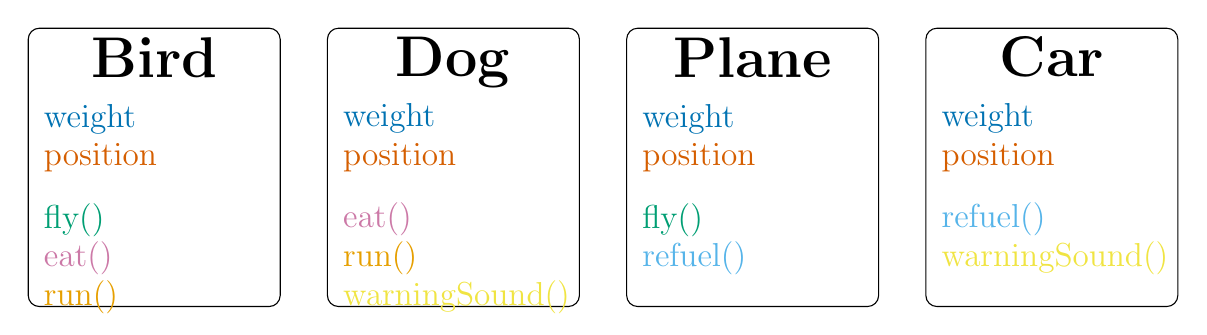
\begin{tikzpicture}
            \tikzset{obj/.style={draw, rounded corners, align=left, text width=2.8cm, minimum width=3.2cm, font=\large}}


            \node[obj] (bird) at (0,0) {
                \begin{minipage}[t][3.3cm][t]{2.8cm}
                    \centering\textbf{\huge Bird}\par\vspace{4pt}
                    \raggedright
                    \textcolor{ecsWeightColor}{weight}\\
                    \textcolor{ecsPositionColor}{position}\\[0.3cm]
                    \textcolor{ecsFlyColor}{fly()}\\
                    \textcolor{ecsEatColor}{eat()}\\
                    \textcolor{ecsRunColor}{run()}\\

                \end{minipage}
            };

            \node[obj] (dog) at (3.8,0) {
                \begin{minipage}[t][3.3cm][t]{2.8cm}
                    \centering\textbf{\huge Dog}\par\vspace{4pt}
                    \raggedright
                    \textcolor{ecsWeightColor}{weight}\\
                    \textcolor{ecsPositionColor}{position}\\[0.3cm]
                    \textcolor{ecsEatColor}{eat()}\\
                    \textcolor{ecsRunColor}{run()}\\
                    \textcolor{ecsWarningColor}{warningSound()}
                \end{minipage}
            };

            \node[obj] (plane) at (7.6,0) {
                \begin{minipage}[t][3.3cm][t]{2.8cm}
                    \centering\textbf{\huge Plane}\par\vspace{4pt}
                    \raggedright
                    \textcolor{ecsWeightColor}{weight}\\
                    \textcolor{ecsPositionColor}{position}\\[0.3cm]
                    \textcolor{ecsFlyColor}{fly()}\\
                    \textcolor{ecsRefuelColor}{refuel()}
                \end{minipage}
            };

            \node[obj] (car) at (11.4,0) {
                \begin{minipage}[t][3.3cm][t]{2.8cm}
                    \centering\textbf{\huge Car}\par\vspace{4pt}
                    \raggedright
                    \textcolor{ecsWeightColor}{weight}\\
                    \textcolor{ecsPositionColor}{position}\\[0.3cm]
                    \textcolor{ecsRefuelColor}{refuel()}\\
                    \textcolor{ecsWarningColor}{warningSound()}
                \end{minipage}
            };
        \end{tikzpicture}
    \end{figure}

\end{frame}
\subsection{Naive Solution: Inheritance}

\begin{frame}
    \frametitle{\insertsubsection}
    \begin{figure}
        \centering
        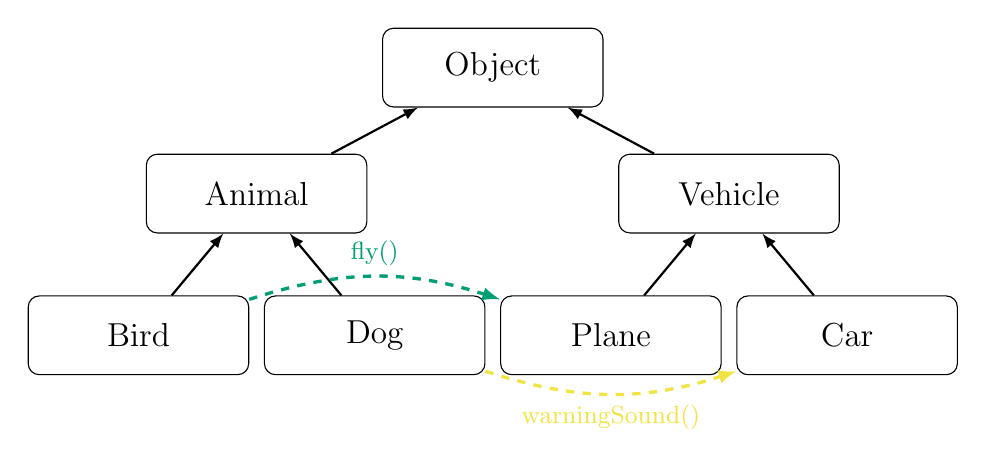
\begin{tikzpicture}
            \tikzset{cls/.style={draw, rounded corners, minimum width=2.8cm, minimum height=1.0cm, align=center, font=\large}}

            \node[cls] (object) at (0,2.8) {Object};

            \node[cls] (animal) at (-3,1.2) {Animal};
            \node[cls] (vehicle) at (3,1.2) {Vehicle};

            \node[cls] (bird) at (-4.5,-0.6) {Bird};
            \node[cls] (dog) at (-1.5,-0.6) {Dog};
            \node[cls] (plane) at (1.5,-0.6) {Plane};
            \node[cls] (car) at (4.5,-0.6) {Car};

            \draw[-latex, thick] (animal) -- (object);
            \draw[-latex, thick] (vehicle) -- (object);

            \draw[-latex, thick] (bird) -- (animal);
            \draw[-latex, thick] (dog) -- (animal);
            \draw[-latex, thick] (plane) -- (vehicle);
            \draw[-latex, thick] (car) -- (vehicle);

            \draw[-latex, very thick, dashed, color=ecsFlyColor, bend left=18] (bird) to node[midway, above, sloped, text=ecsFlyColor] {\small fly()} (plane);
            \draw[-latex, very thick, dashed, color=ecsWarningColor, bend right=18] (dog) to node[midway, below, sloped, text=ecsWarningColor] {\small warningSound()} (car);
        \end{tikzpicture}
    \end{figure}

    \uncover<2->{
        \begin{note}{Problem}
            \begin{itemize}
                \item Arbitrary grouping of properties and behaviors often breaks simple hierarchy
                \item Consequences: code duplication \& complex inheritance structures
            \end{itemize}
        \end{note}
    }
\end{frame}

\subsection{Concept}

\begin{frame}
    \frametitle{\insertsection{} -- \insertsubsection{}}

    \begin{fancycolumns}[widths={40,60}]
        \begin{definition}{Entity-Component-System}
            \begin{itemize}
                \item Three core concepts: Entity, Component, System
                \item \emph{Entity}: Unique incarnation of an object, typically just an ID
                \item \emph{Component}: Data container representing a property of an entity
                \item \emph{System}: Logic that operates on entities with specific components, manipulating their data
            \end{itemize}
        \end{definition}
        \nextcolumn
        \defaultentitycomponentsystem{}
    \end{fancycolumns}
\end{frame}

\subsection{Example}

\begin{frame}
    \frametitle{\insertsection{} -- \insertsubsection{}}
\begin{figure}
            \centering
            \begin{tikzpicture}
                \tikzset{
                    entity/.style={draw, rounded corners, minimum width=2.3cm, minimum height=0.75cm, align=center, fill=black!30, font=\small},
                    system/.style={draw, rounded corners, minimum width=2.7cm, minimum height=0.8cm, align=center, fill=black!30, font=\small\bfseries},
                    comp/.style={draw, rounded corners, minimum width=2.4cm, minimum height=0.7cm, align=center, font=\small\bfseries}
                }

                % Entities
                \node[entity] (e1) at (0,2.2) {Entity: Bird};
                \node[entity, below=2mm of e1] (e2) {Entity: Dog};
                \node[entity, below=2mm of e2] (e3) {Entity: Plane};
                \node[entity, below=2mm of e3] (e4) {Entity: Car};

                % Components
                \node[comp, draw=ecsWeightColor, fill=ecsWeightColor!18, text=ecsWeightColor] (c1) at (5,2.8) {WeightComponent};
                \node[comp, draw=ecsPositionColor, fill=ecsPositionColor!18, text=ecsPositionColor, below=2mm of c1] (c2) {PositionComponent};
                \node[comp, draw=ecsFlyColor, fill=ecsFlyColor!18, text=ecsFlyColor, below=2mm of c2] (c3) {FlyComponent};
                \node[comp, draw=ecsEatColor, fill=ecsEatColor!18, text=ecsEatColor, below=2mm of c3] (c4) {EatComponent};
                \node[comp, draw=ecsRefuelColor, fill=ecsRefuelColor!18, text=ecsRefuelColor, below=2mm of c4] (c5) {RefuelComponent};
                \node[comp, draw=ecsRunColor, fill=ecsRunColor!18, text=ecsRunColor, below=2mm of c5] (c6) {RunComponent};
                \node[comp, draw=ecsWarningColor, fill=ecsWarningColor!18, text=ecsWarningColor, below=2mm of c6] (c7) {WarningComponent};

                % Systems
                \node[system] (s1) at (10,1.8) {MovementSystem};
                \node[system, below=5mm of s1] (s2) {ResourceSystem};

                % Entity -> Component membership
                \draw[-latex, thick] (e1.east) -- (c1.west);
                \draw[-latex, thick] (e1.east) -- (c2.west);
                \draw[-latex, thick] (e1.east) -- (c3.west);
                \draw[-latex, thick] (e1.east) -- (c4.west);
                \draw[-latex, thick] (e1.east) -- (c6.west);

                \draw[-latex, thick] (e2.east) -- (c1.west);
                \draw[-latex, thick] (e2.east) -- (c2.west);
                \draw[-latex, thick] (e2.east) -- (c4.west);
                \draw[-latex, thick] (e2.east) -- (c6.west);
                \draw[-latex, thick] (e2.east) -- (c7.west);

                \draw[-latex, thick] (e3.east) -- (c1.west);
                \draw[-latex, thick] (e3.east) -- (c2.west);
                \draw[-latex, thick] (e3.east) -- (c3.west);
                \draw[-latex, thick] (e3.east) -- (c5.west);

                \draw[-latex, thick] (e4.east) -- (c1.west);
                \draw[-latex, thick] (e4.east) -- (c2.west);
                \draw[-latex, thick] (e4.east) -- (c5.west);
                \draw[-latex, thick] (e4.east) -- (c7.west);

                % Systems operating on components
                \draw[-latex, thick, dashed] (s1.west) -- (c2.east);
                \draw[-latex, thick, dashed] (s1.west) -- (c3.east);
                \draw[-latex, thick, dashed] (s1.west) -- (c6.east);
                \draw[-latex, thick, dashed] (s2.west) -- (c1.east);
                \draw[-latex, thick, dashed] (s2.west) -- (c4.east);
                \draw[-latex, thick, dashed] (s2.west) -- (c5.east);
                \draw[-latex, thick, dashed] (s2.west) -- (c7.east);
            \end{tikzpicture}
        \end{figure}
    

\end{frame}

\subsection{Considerations}

\begin{frame}
    \frametitle{\insertsection{} -- \insertsubsection{}}

        \begin{fancycolumns}[widths={40,60}]
            \begin{motivation}{Advantages}
                \begin{itemize}
                    \item Flexible composition of properties and behaviors
                    \item Improved code reuse and separation of concerns
                    \item Improved memory layout $\rightarrow$ performance benefits
                \end{itemize}
            \end{motivation}
            \begin{note}{Disadvantages}
                \begin{itemize}
                    \item More complex design
                \end{itemize}
            \end{note}
            \nextcolumn
            \defaultentitycomponentsystem{}
        \end{fancycolumns}

    

\end{frame}
